\documentclass{article}
\usepackage{graphicx, fancyhdr, amsmath}
\usepackage[margin=0.6in, top=1in]{geometry}
\usepackage{float}
\usepackage[absolute, overlay]{textpos}
\usepackage[colorlinks=true, linkcolor=blue]{hyperref}

\pagestyle{fancy}
\fancyhf{}
\renewcommand{\headrulewidth}{0pt}

\fancyhead[L]{
\begin{textblock*}{2cm}(0.3in,0.1in)  % {block width} (x-coordinate, y-coordinate)
    
\includegraphics[width=2cm]{NEW LOGO.png}  % Example image placeholder
\end{textblock*}
}
\fancyhead[R]{Math Success Program, UCLA}
\fancyfoot[R]{Created for the MSP by Asmi Kawatkar}

\fancypagestyle{plain}{
}


\title{Review Sheet: Hyperbolic Functions}
\date{}
\author{}

\begin{document}
\maketitle
\vspace{-0.75in}
\section*{Content Review}
\subsection*{Overview}

\textit{Basic Definitions}

$$ \sinh x = \frac{e^x - e^{-x}}{2}$$
$$ \cosh x = \frac{e^x + e^{-x}}{2}$$

For the remaining hyperbolic functions, apply the same relationships that you already know for basic trigonometry:

\begin{eqnarray*}
    \tanh x &=& \frac{\sinh x}{\cosh x}\\
    \coth x &=& \frac{\cosh x}{\sinh x}\\
    \text{sech} x &=& \frac{1}{\cosh x} \\
    \text{csch} x &=& \frac{1}{\sinh x}
\end{eqnarray*}

\noindent\textit{Basic Properties}
\\Notice that the hyperbolic functions have effectively the same properties as their trigonometric counterparts

$$\sinh (-x) = -\sinh x$$
$$\cosh (x) = \cosh x$$
$$\tanh (-x) = -\tanh x$$
$$\coth (-x) = -\coth x$$
$$\text{sech} (-x) = \text{sech}x$$
$$\text{csch} (-x) = -\text{csch}x$$

\vspace{0.2in}
\noindent \textit{Identities}
\\ Note that the signs for these identities are not the same as trigonometric identities. Be very careful of which signs you use. 

$$\cosh^2 x - \sinh^2 x = 1$$
$$\tanh^2 x + \text{sech}^2 x = 1$$

\noindent Additive identities for hyperbolic functions can also be derived in a similar way to trigonometric functions. 

$$\sinh(x+y) = \sinh x \cosh y + \cosh x \sinh y$$
$$\cosh(x+y) = \cosh x \cosh y + \sinh x \sinh y$$

\noindent Double angle identities for hyperbolic functions are as follows:

$$\sinh{2x} = 2 \sinh x \cosh x$$
$$\cosh{2x} = \cosh^2 x + \sinh^2 x$$

\noindent\textit{Inverse Hyperbolic Functions}
$$\sinh^{-1}(x) = \ln (x+\sqrt{x^2 + 1})$$
$$\cosh^{-1}(x) = \ln (x+\sqrt{x^2 - 1})$$
$$\tanh^{-1}(x) = \frac{1}{2}\ln \frac{1+x}{1-x}$$

\noindent An example of deriving these inverses is shown below:

\noindent Note: $y = \sinh x \Longleftrightarrow \sinh^{-1} y = x$\\

Thus, 
$$y = \sinh x = \frac{e^x - e^{-x}}{2} \longleftrightarrow 2y = e^x - e^{-x}$$
\begin{eqnarray*}
    &\implies& 2y = e^x - \frac{1}{e^x} \\
    &\implies& 2y = \frac{e^{2x} - 1}{e^x}\\
    &\implies& 2ye^x = e^{2x} - 1 \\
    &\implies& e^{2x} - 2ye^x - 1 = 0 \hspace{0.5in} \text{ Solve this by treating $e^x$ as a variable and applying the quadratic formula}\\
    &\implies& e^x = \frac{2y \pm \sqrt{4y^2 +4}}{2}  = y \pm \sqrt{y^2 + 1} \hspace{0.5in} \text{Since log only takes positive numbers, choose the positive sign}\\
    &\implies& x = \ln (y + \sqrt{y^2 + 1})\\
    &\implies& \sinh^{-1}(y) = \ln(y+\sqrt{y^2 + 1})
\end{eqnarray*}

\vspace{0.2in}
\noindent\textit{Derivatives of Hyperbolic Functions}

\begin{eqnarray*}
    \frac{d}{dx} \sinh x &=& \cosh x \\
    \frac{d}{dx} \cosh x &=& \sinh x \\
    \frac{d}{dx} \tanh x &=& \text{sech}^2 x \\
    \frac{d}{dx} \coth x &=& \text{csch}^2 x \\
    \frac{d}{dx} \text{sech} x &=& \tanh x \cdot \text{sech} x \\
    \frac{d}{dx} \text{csch} x &=& -\text{coth} x \cdot \text{csch} x\\
\end{eqnarray*}

\subsection*{Resources}


\noindent\textit{Related Rates}
\begin{itemize}
    \item \href{https://www.whitman.edu/mathematics/calculus_online/section04.11.html}{Content: Hyperbolic Functions (Whitman Edu)} 
    \item \href{https://tutorial.math.lamar.edu/classes/calci/DiffHyperFcns.aspx}{Content: Derivatives of Hyperbolic Functions (Paul's Online Notes)}
    \item \href{https://www.mathcentre.ac.uk/resources/workbooks/mathcentre/hyperbolicfunctions.pdf}{Content: Hyperbolic Functions Explained (MathCenter UK)}
    \item \href{https://youtu.be/PJRSu0Vf0r0}{Video: Hyperbolic Trig Functions, Basic Introduction (Organic Chemistry Tutor, 10 min)}
    \item \href{https://youtu.be/w_UEjfADQQc}{Video: Graphs of Hyperbolic Trig Functions (Organic Chemistry Tutor, 23 min)}
    \item \href{https://youtu.be/va09U91xHxA}{Video: Evaluating Hyperbolic Trig Functions (Organic Chemistry Tutor, 9min)}
    \item \href{https://youtu.be/m9nwdn55Z2w}{Video: Hyperbolic Trig Identities (Organic Chemistry Tutor, 10 min)}
    \item \href{https://www.cimt.org.uk/projects/mepres/alevel/fpure_ch2.pdf}{Practice Problems: Hyperbolic Functions}
    \item \href{https://s3.amazonaws.com/calculus-worksheets/calculus-2-tutor/Calculus+2+Tutor+-+Worksheet+3+-+Hyperbolic+Functions.pdf}{Practice Problems: Hyperbolic Function (Calculus)}
\end{itemize}

\subsection*{Acknowledgement}
Questions in the Worked Problems section of this sheet have been taken from external sources that have been linked where appropriate. All solutions have been created independently.

\pagebreak
\section*{Worked Problems}
\label{WorkedProblems}

\noindent Find the derivative of the following functions: 
\newline(\href{https://www.deanza.edu/faculty/kleincharles/documents/HyperbolicFunctionsProblems.pdf}{Source})
\begin{enumerate}
    \item $$y = \tanh x$$
    \begin{figure}[H]
        \centering
        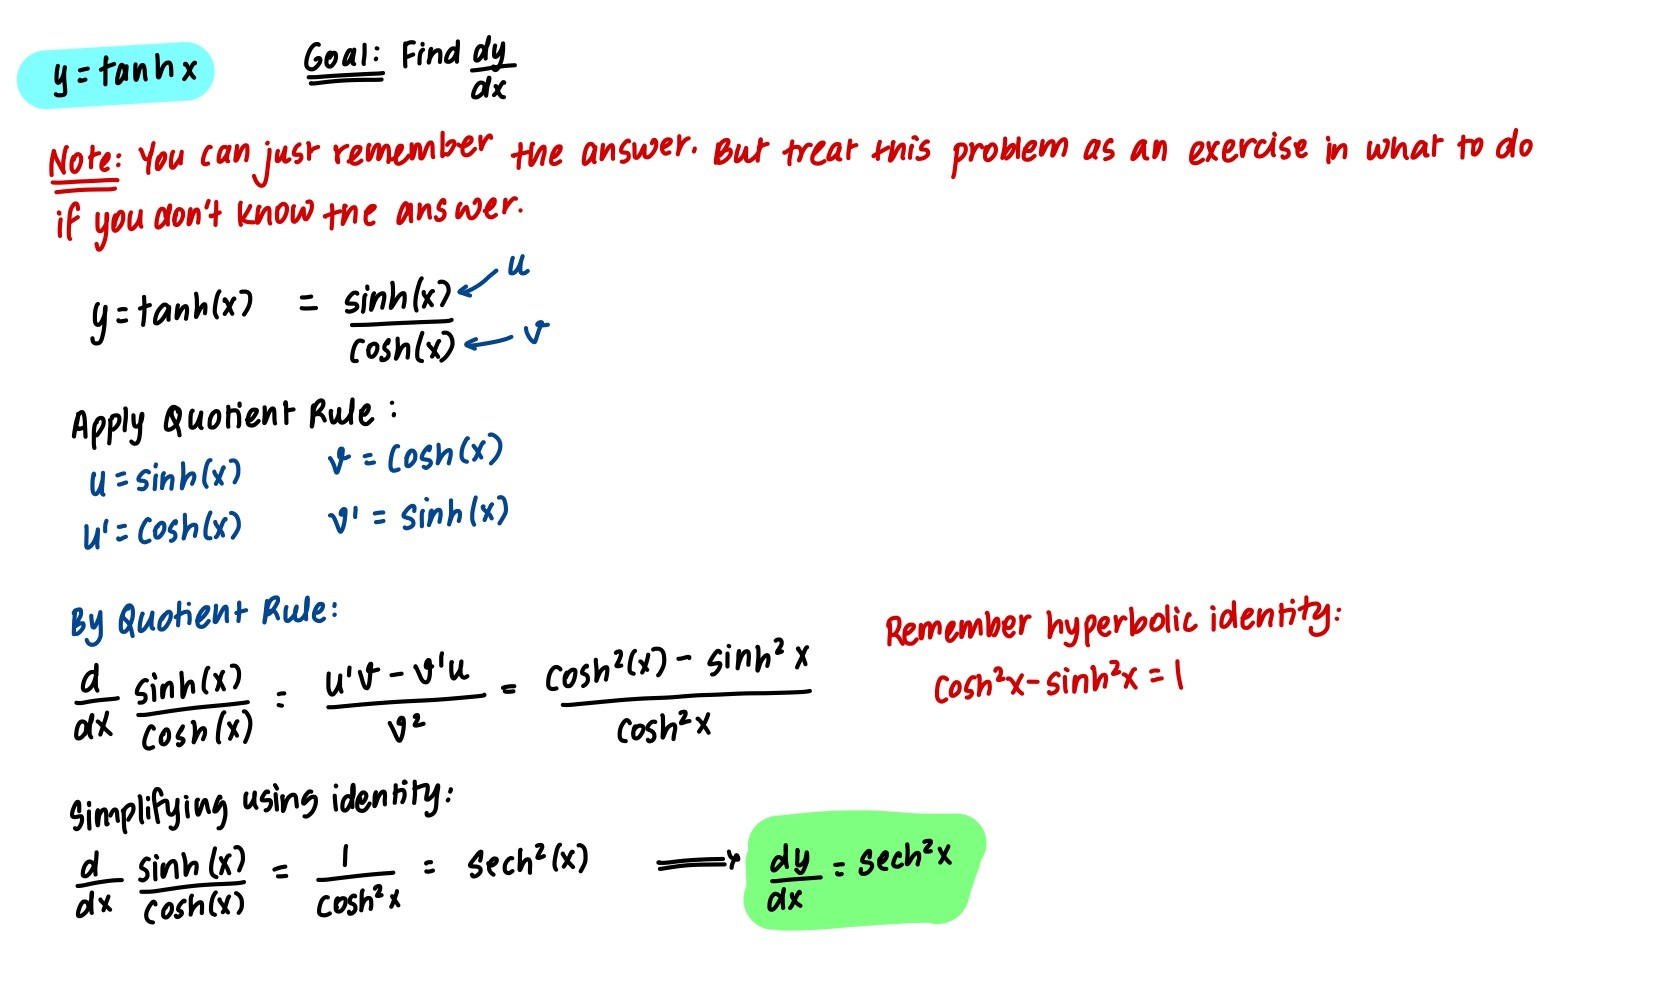
\includegraphics[width=\linewidth]{Q1.jpg}
        \label{fig:Q1}
    \end{figure}
    \item $$y = e^x \cosh x$$
    \begin{figure}[H]
        \centering
        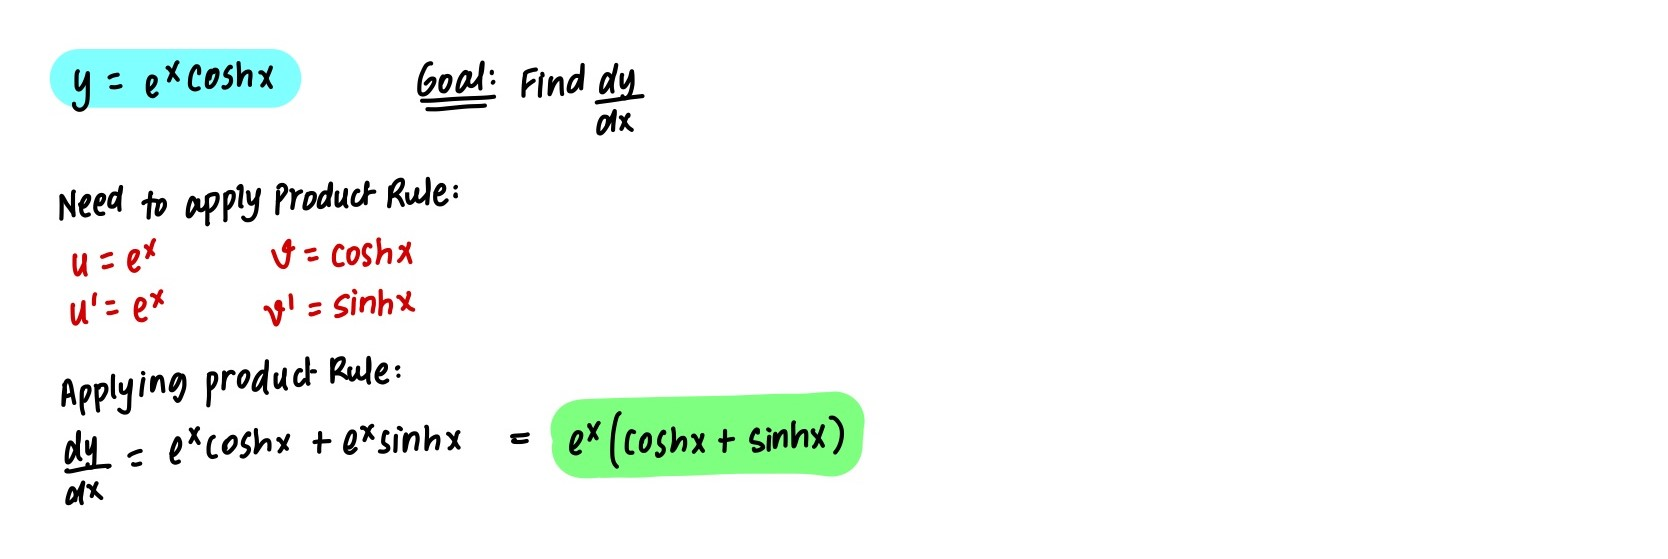
\includegraphics[width=\linewidth]{Q2.jpg}
        \label{fig:Q2}
    \end{figure}
    \item $$y = \cosh{x^3}$$
    \begin{figure}[H]
        \centering
        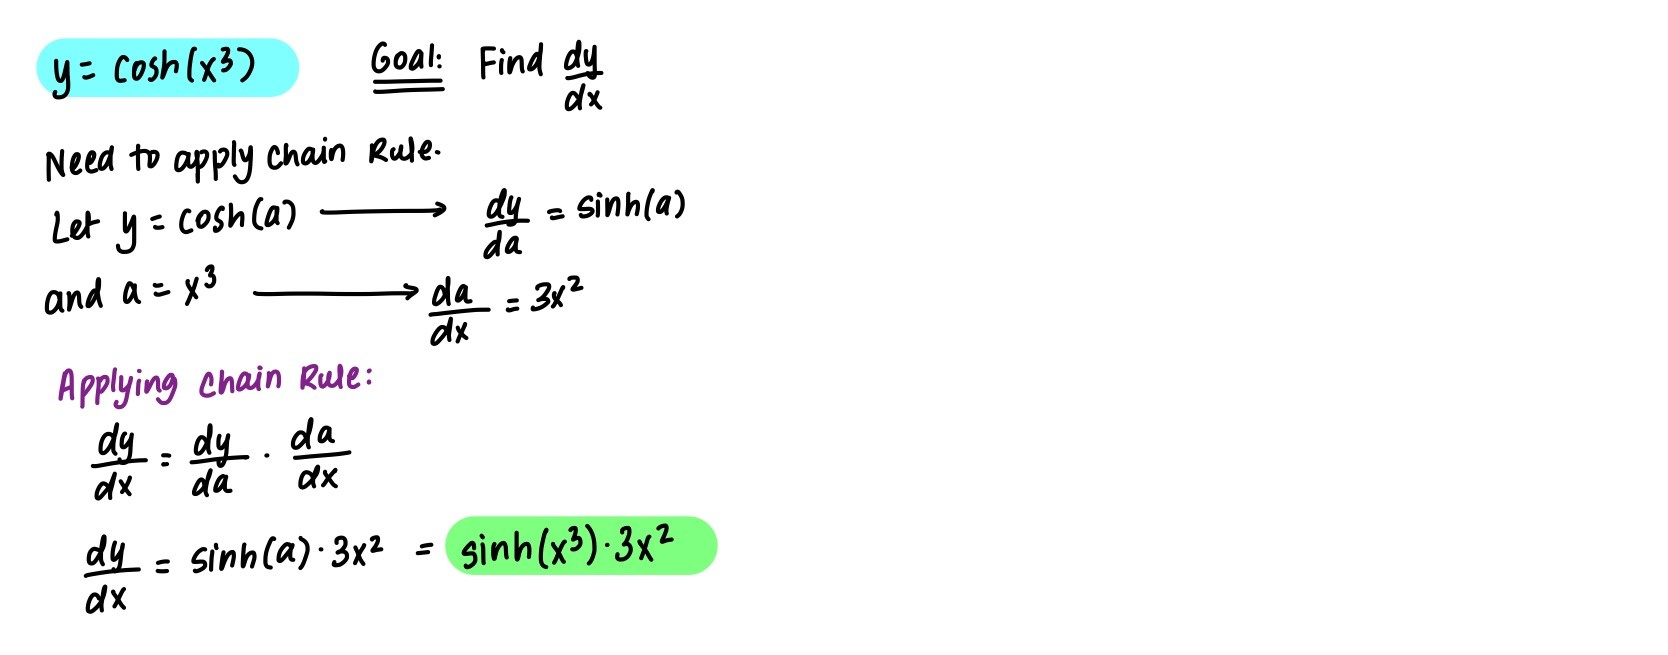
\includegraphics[width=\linewidth]{Q3.jpg}
        \label{fig:Q3}
    \end{figure}
    \item $$y = \cosh{\ln x}$$
    \begin{figure}[H]
        \centering
        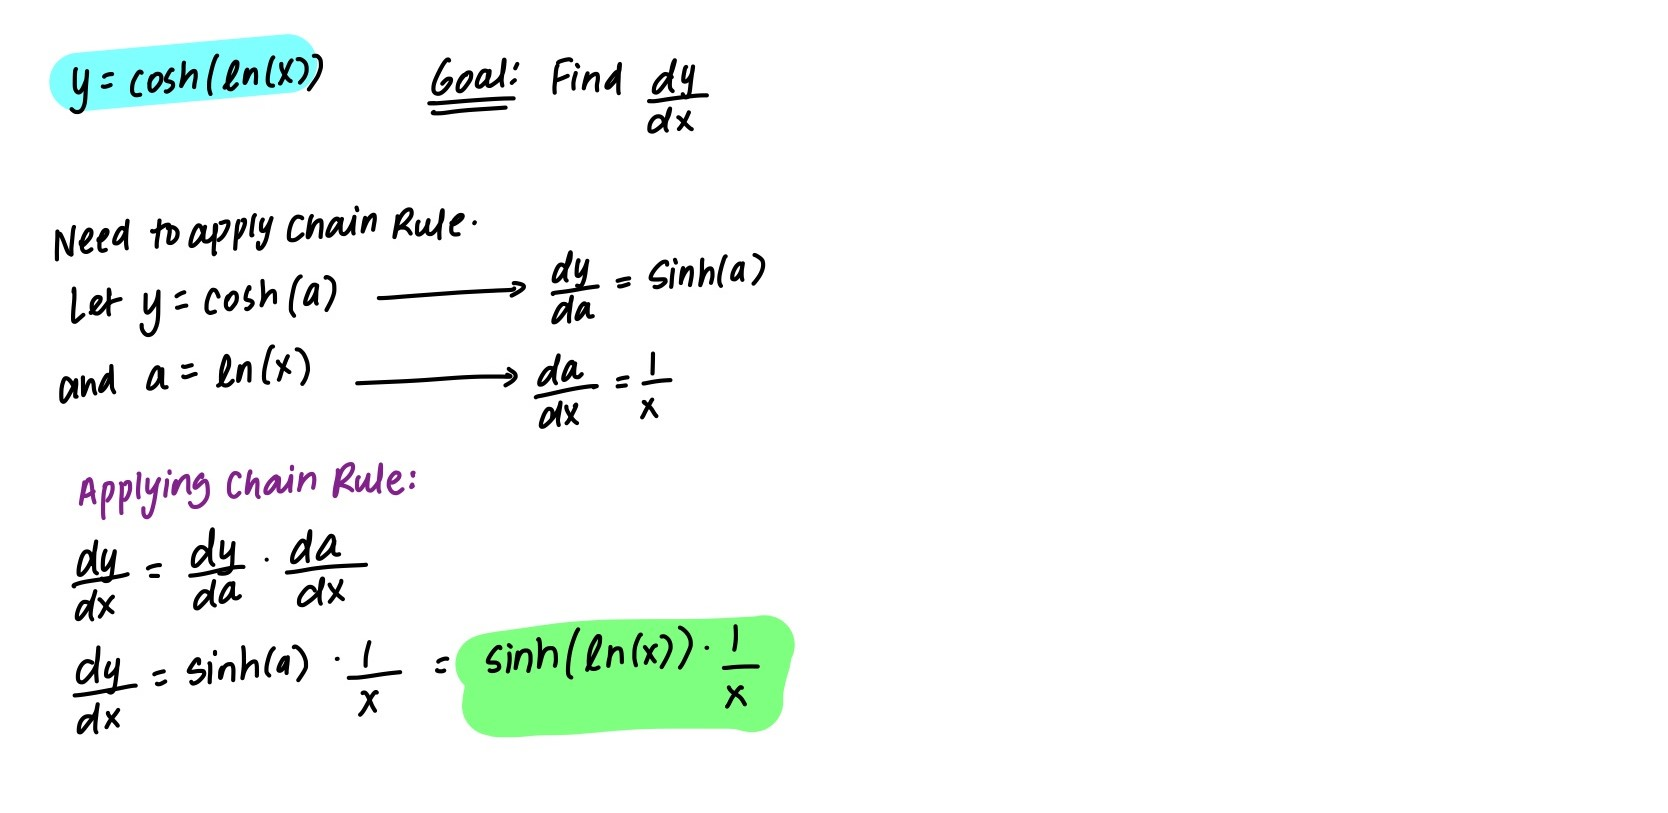
\includegraphics[width=\linewidth]{Q4.jpg}
        \label{fig:Q4}
    \end{figure}
    \newpage
    \item $$y = \sin^{-1}({\tanh{x^2}})$$
    \begin{figure}[H]
        \centering
        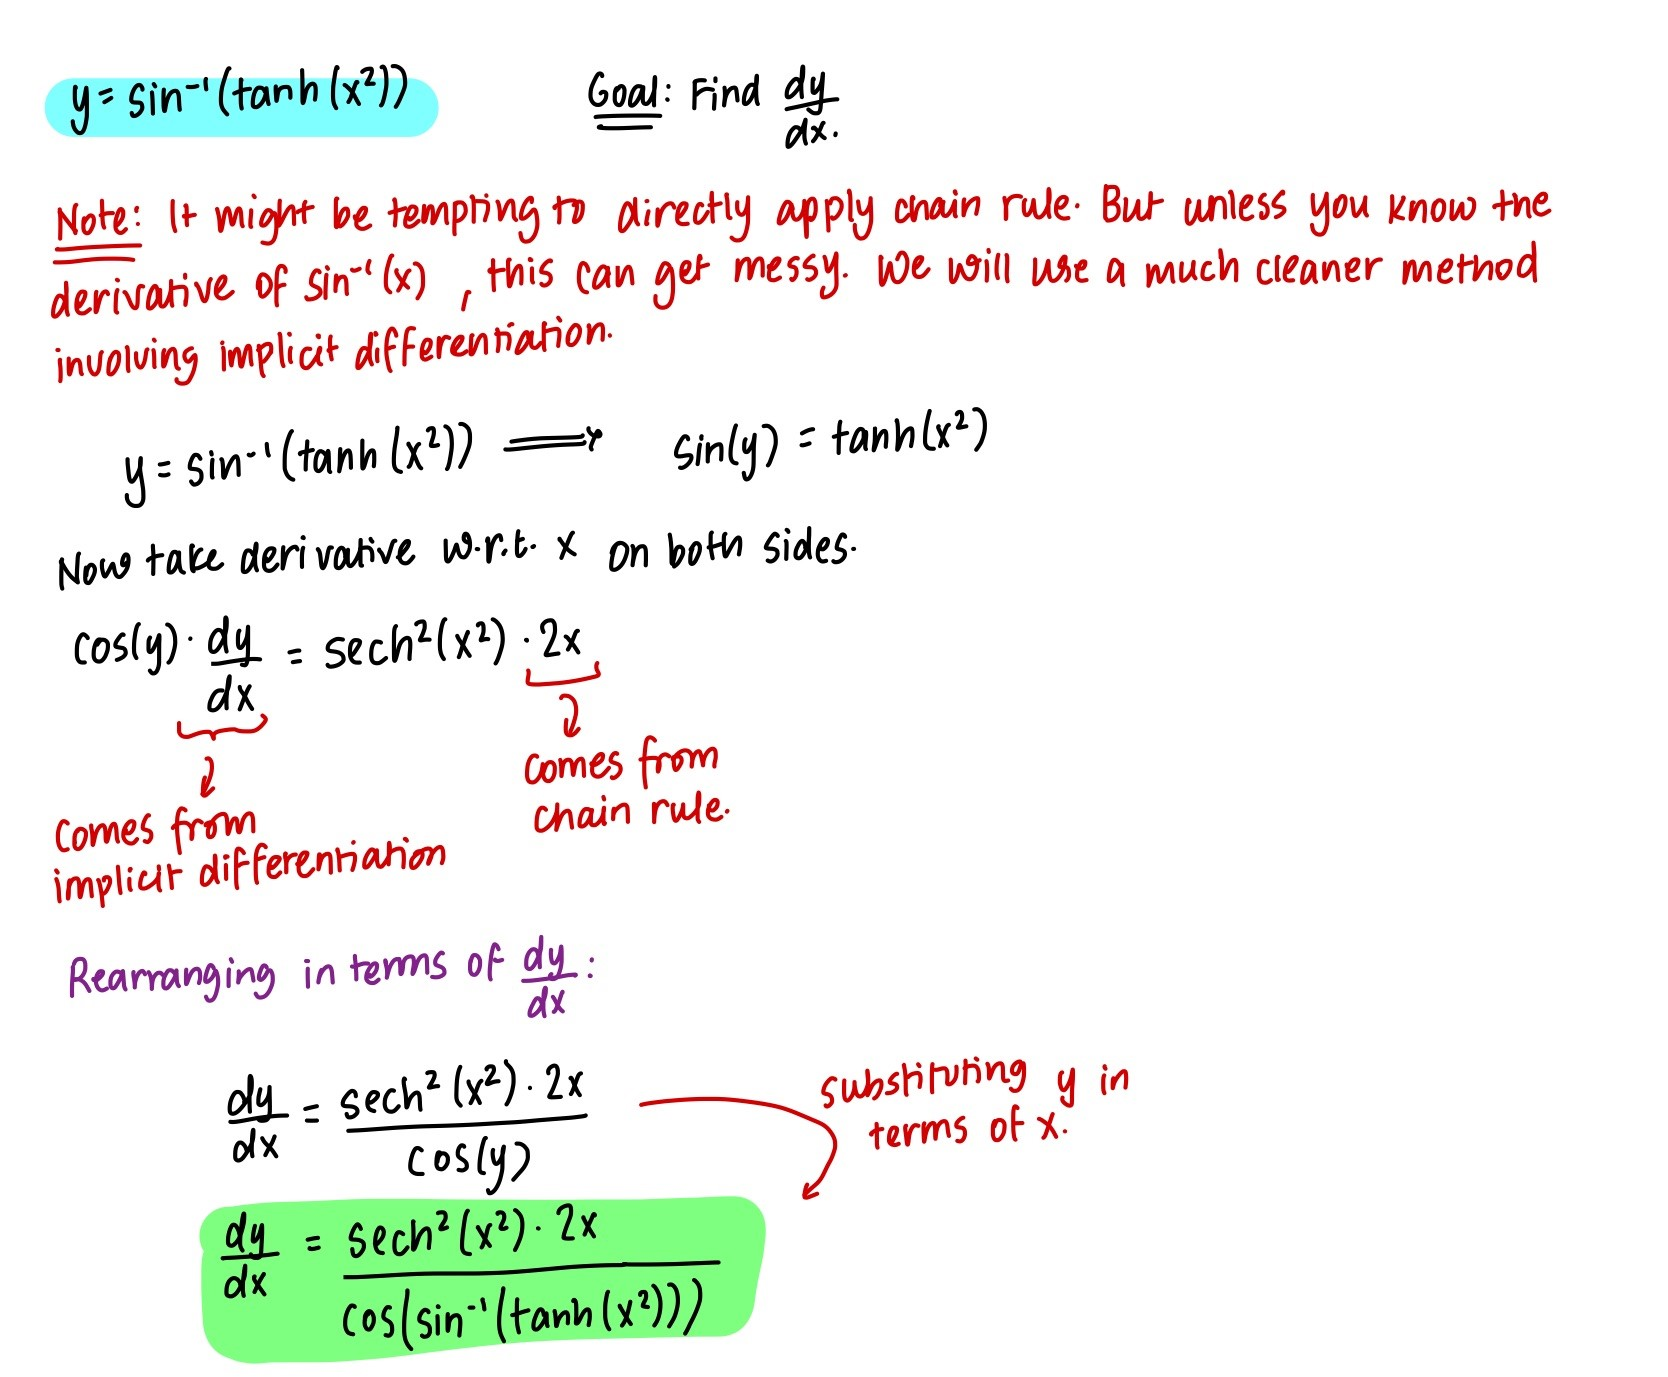
\includegraphics[width=\linewidth]{Q5.jpg}
        \label{fig:Q5}
    \end{figure}
\end{enumerate}

\newpage
\noindent Find the following antiderivatives: 
\newline (\href{https://www.deanza.edu/faculty/kleincharles/documents/HyperbolicFunctionsProblems.pdf}{Source})
\begin{enumerate}
    \item $$\int \sinh^4(x) \cdot \cosh x dx$$
    \begin{figure}[H]
        \centering
        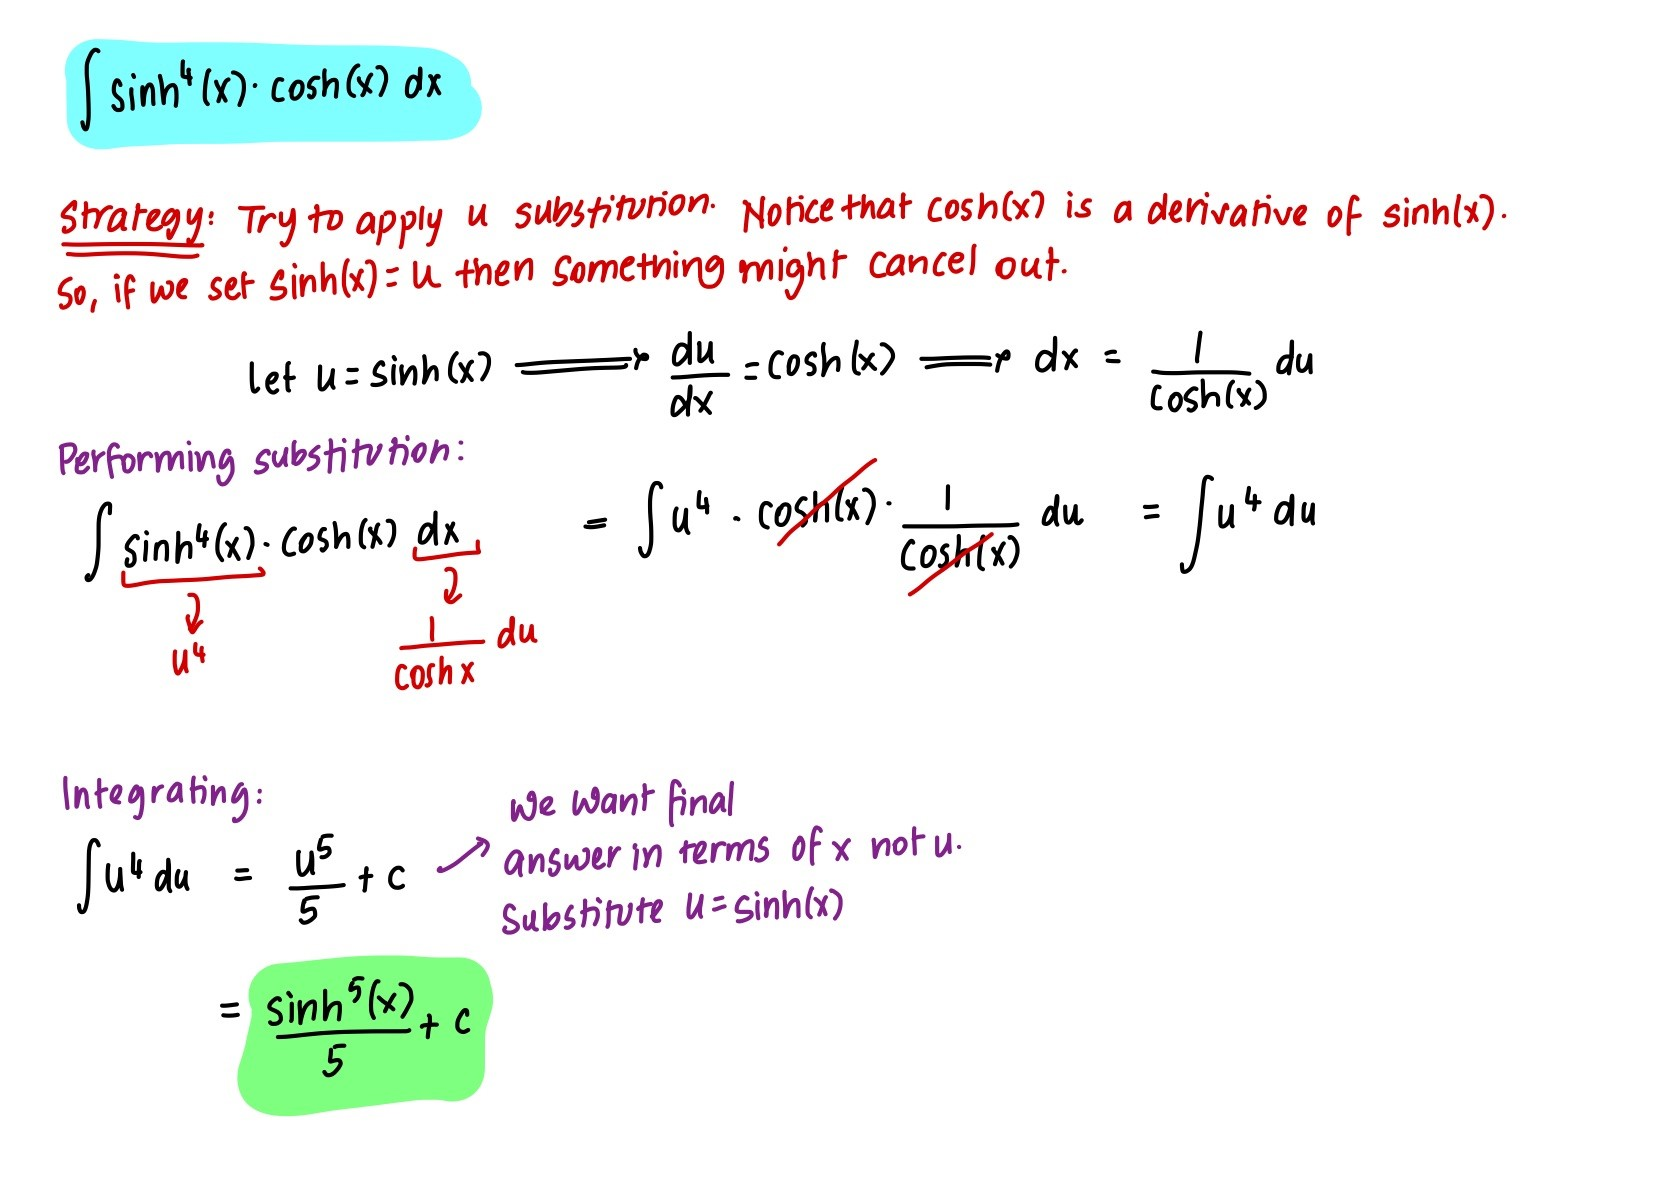
\includegraphics[width=\linewidth]{Q1.1.jpg}
        \label{fig:Q1.1}
    \end{figure}
    \newpage
    \item $$\int e^x \cdot \cosh e^x \cdot \sinh e^x dx$$
    \begin{figure}[H]
        \centering
        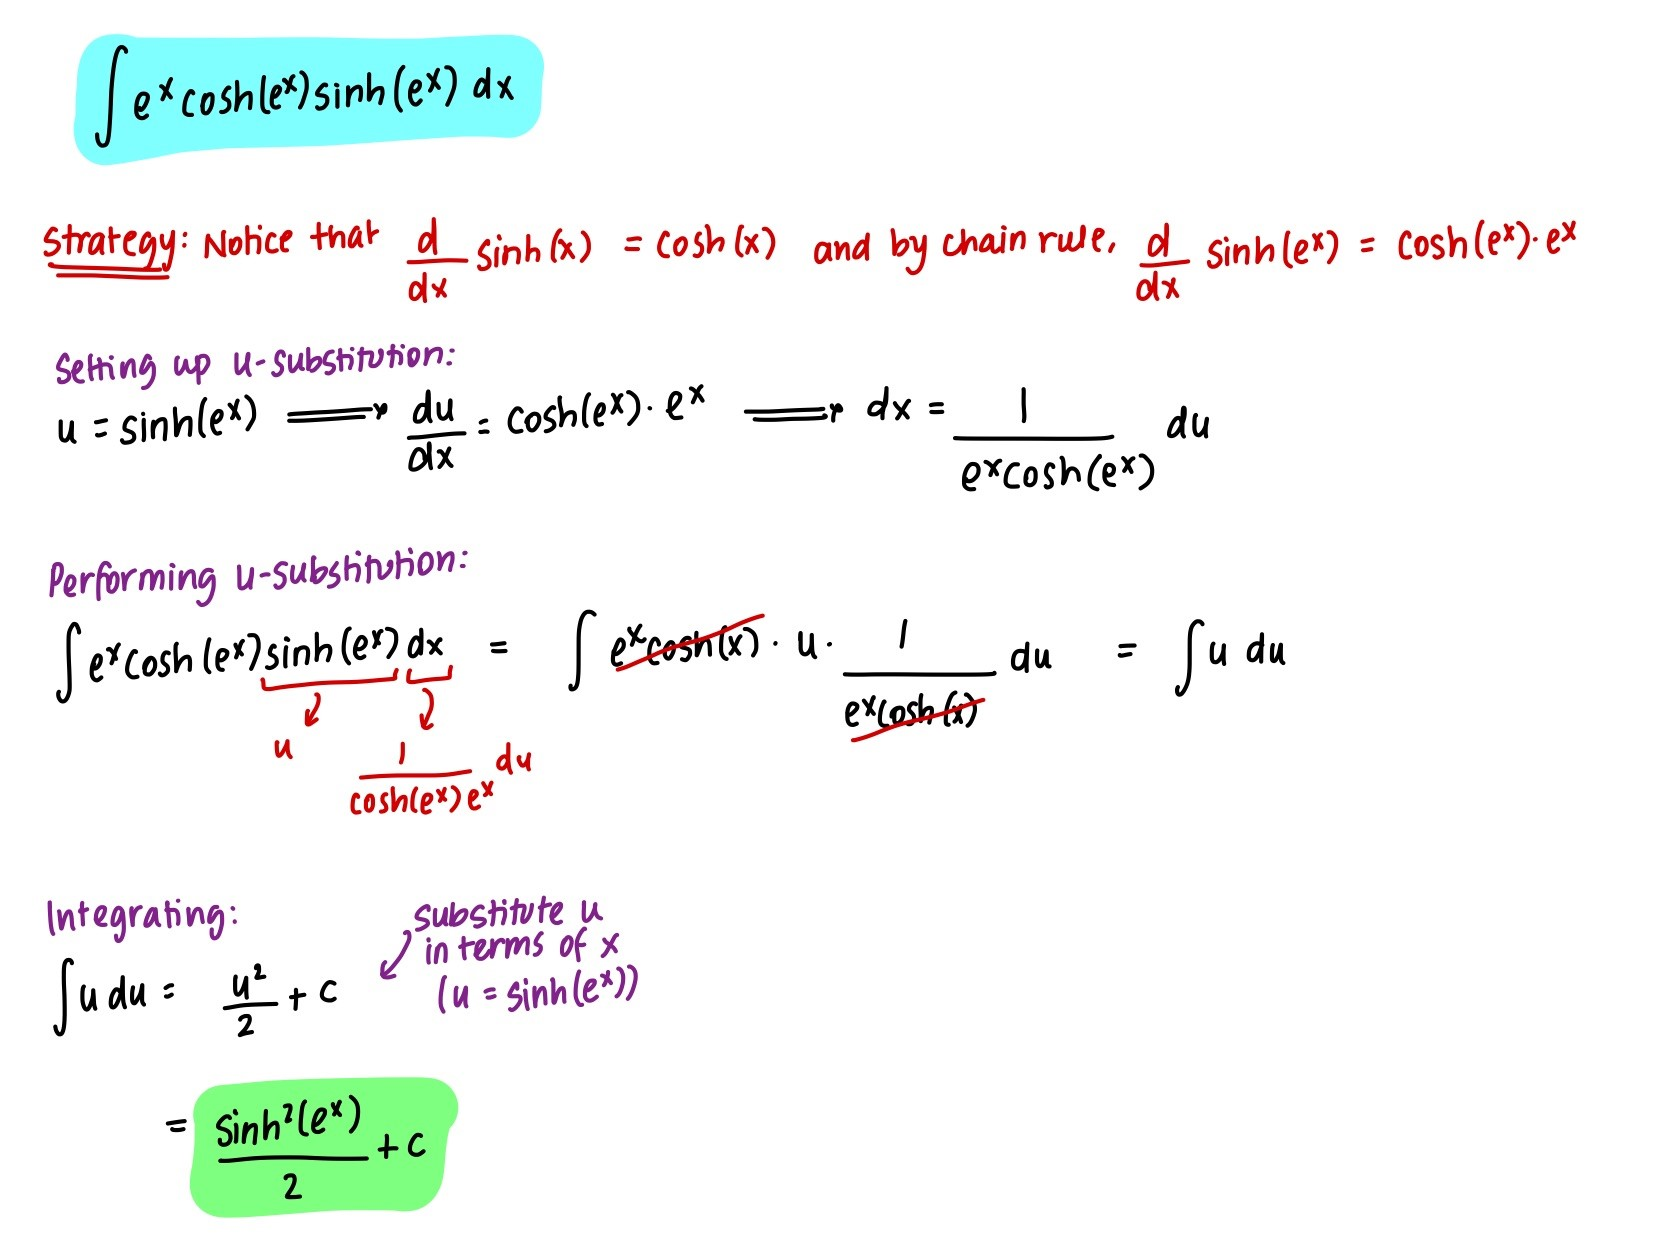
\includegraphics[width=\linewidth]{Q1.2.jpg}
        \label{fig:Q1.2}
    \end{figure}
    \newpage
    \item $$\int \frac{\sinh x}{1 + \cosh x}$$
    \begin{figure}[H]
        \centering
        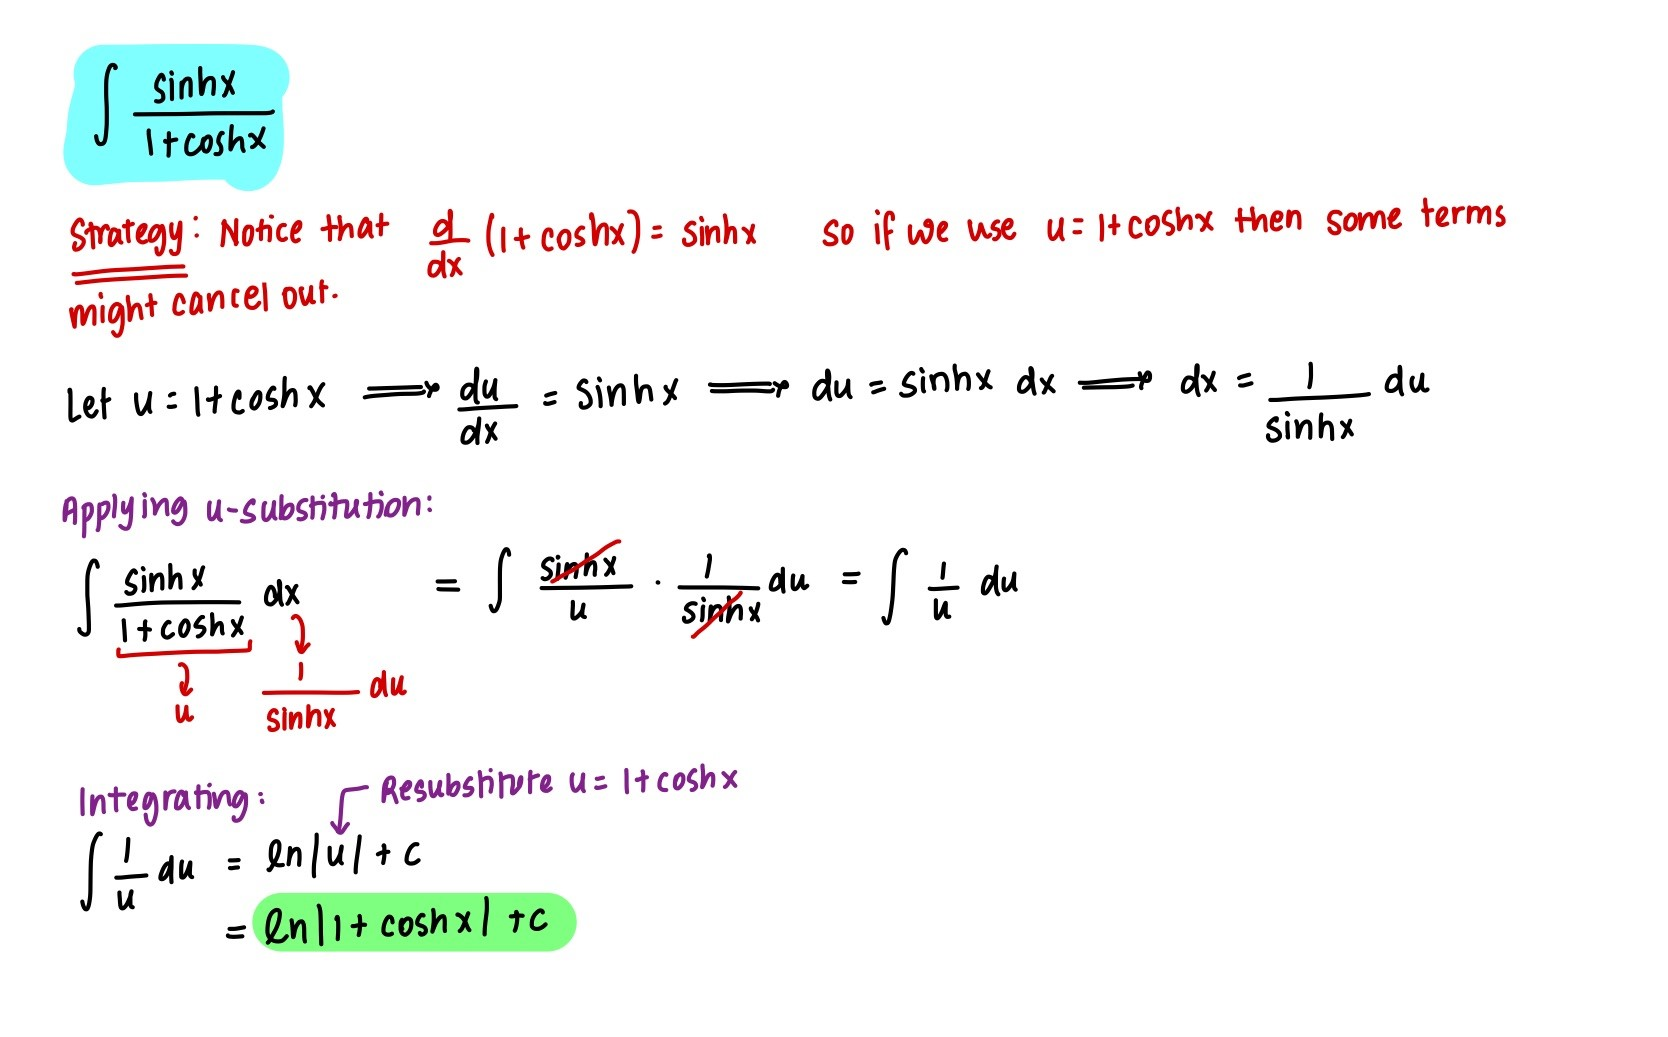
\includegraphics[width=\linewidth]{Q1.3.jpg}
        \label{fig:Q1.3}
    \end{figure}
\end{enumerate}

\newpage \noindent 
Answer the following questions 
\newline (\href{https://www.deanza.edu/faculty/kleincharles/documents/HyperbolicFunctionsProblems.pdf}{Source} and \href{https://www.thomasbury.net/uploads/math117/examples_3.pdf}{Source})
\begin{enumerate}
    \item At what point on the curve $y = \cosh x$ does the tangent to the curve have a slope of 1?
    \begin{figure}[H]
        \centering
        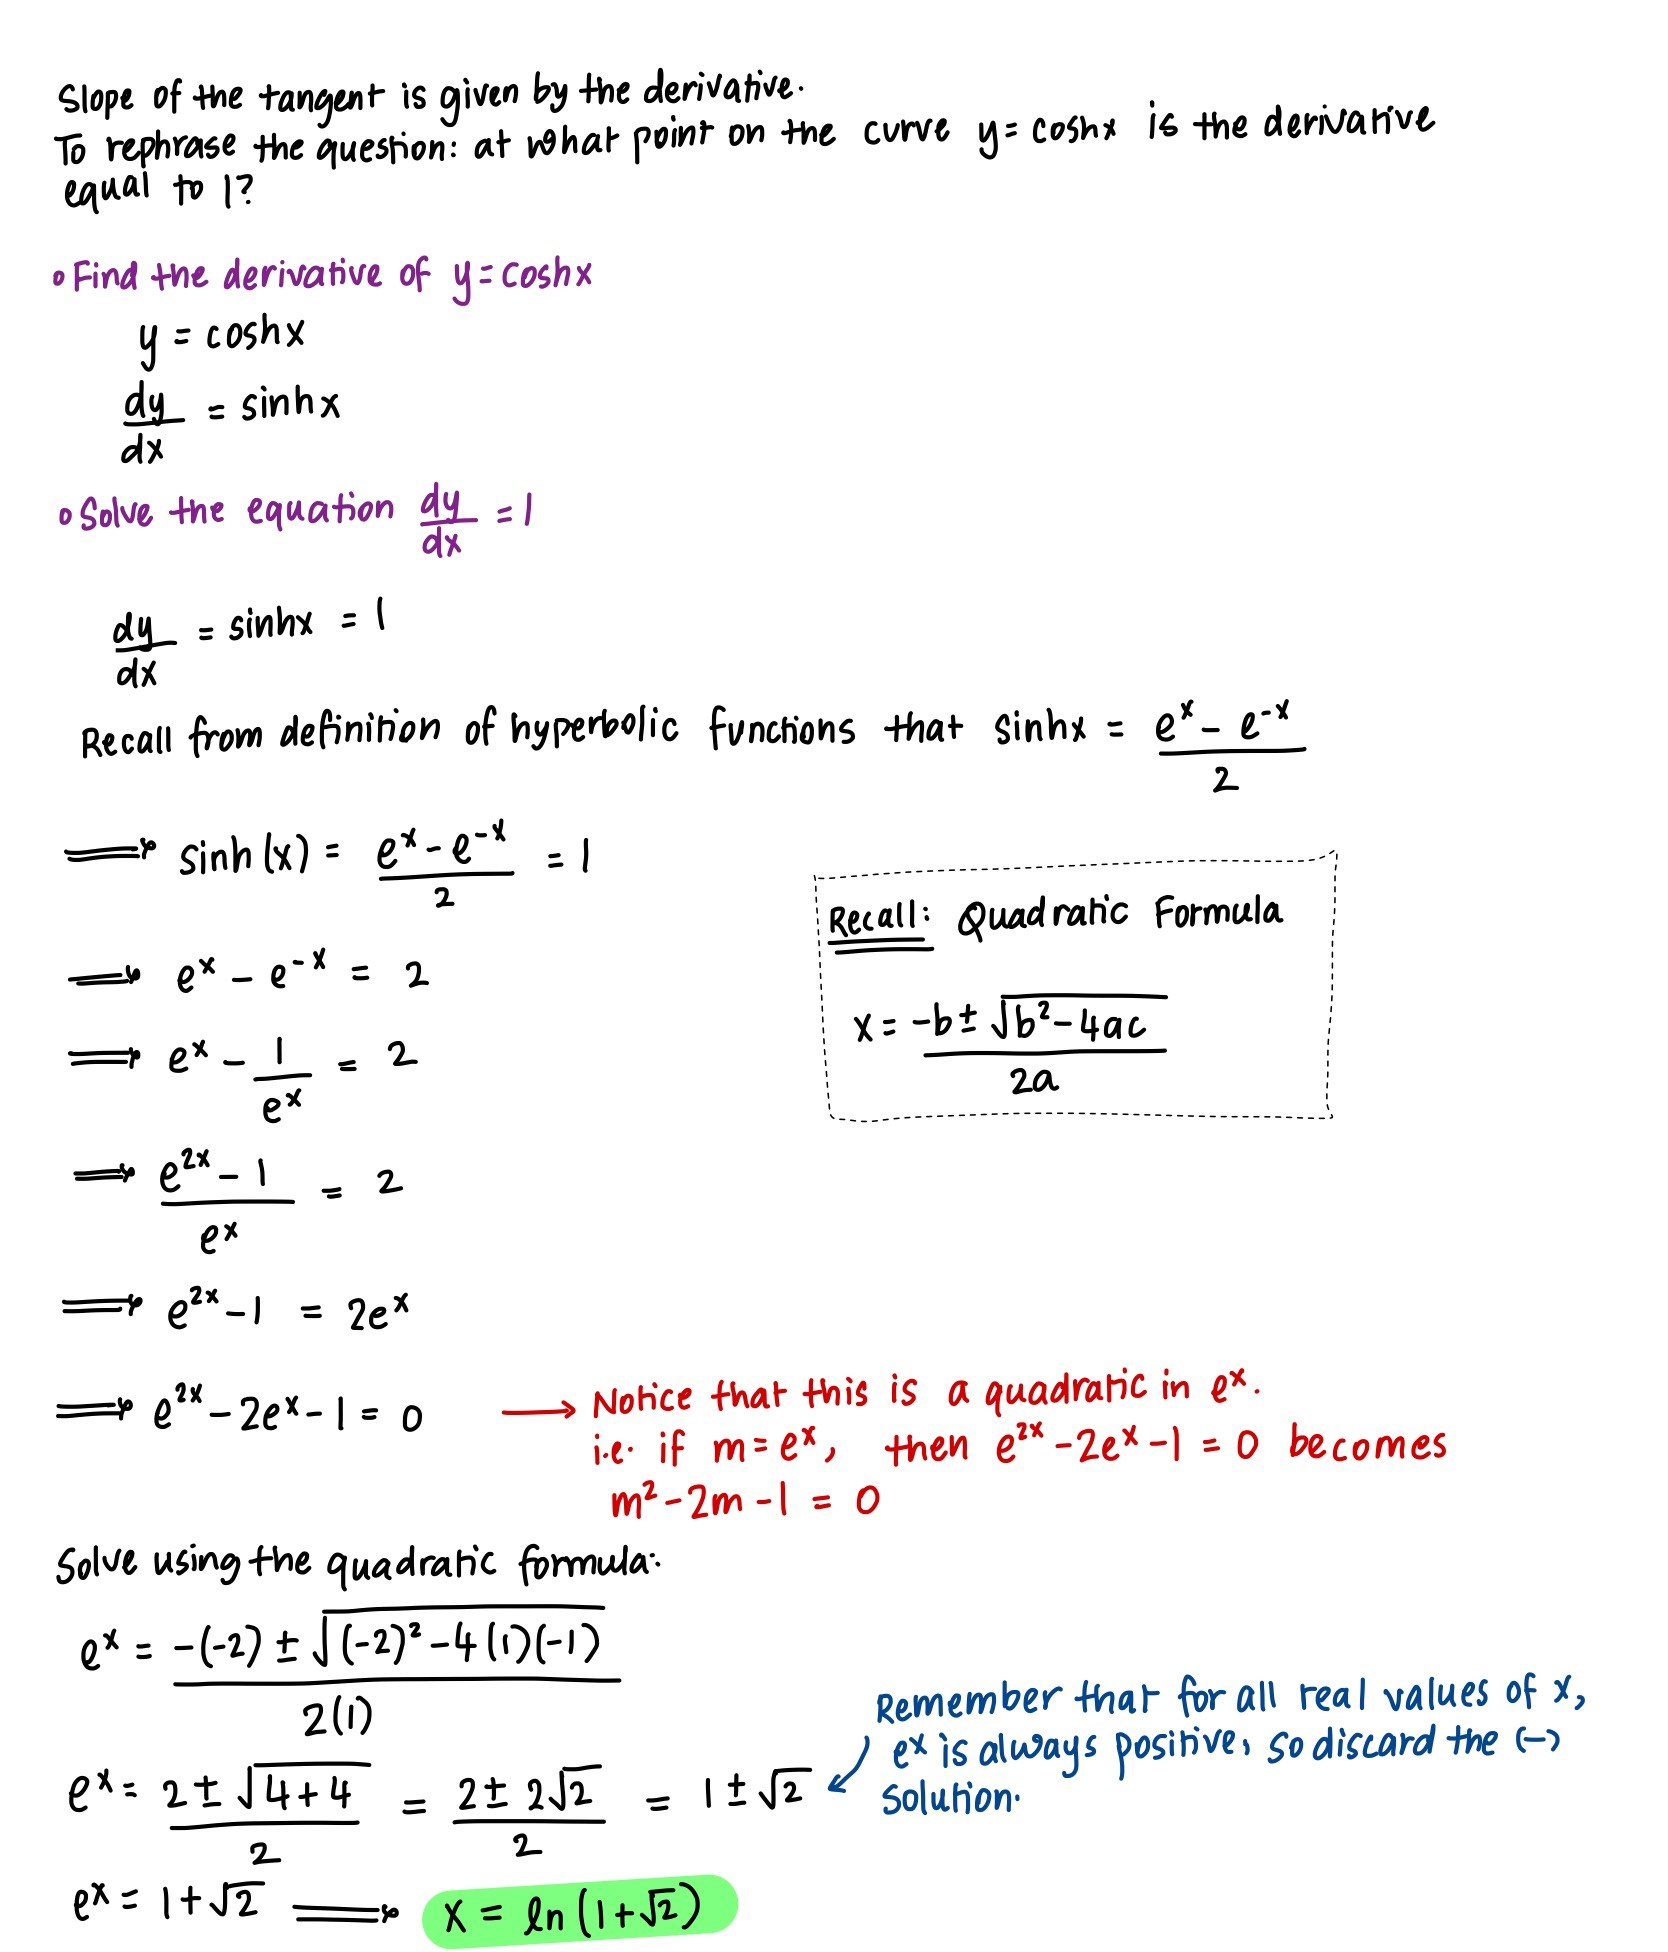
\includegraphics[width=0.95\linewidth]{Q2.1.jpg}
        \label{fig:Q2.1}
    \end{figure}
    \newpage
    \item Show that $$\sinh^{-1} x = \ln(x + \sqrt{x^2 + 1})$$. 
    \begin{figure}[H]
        \centering
        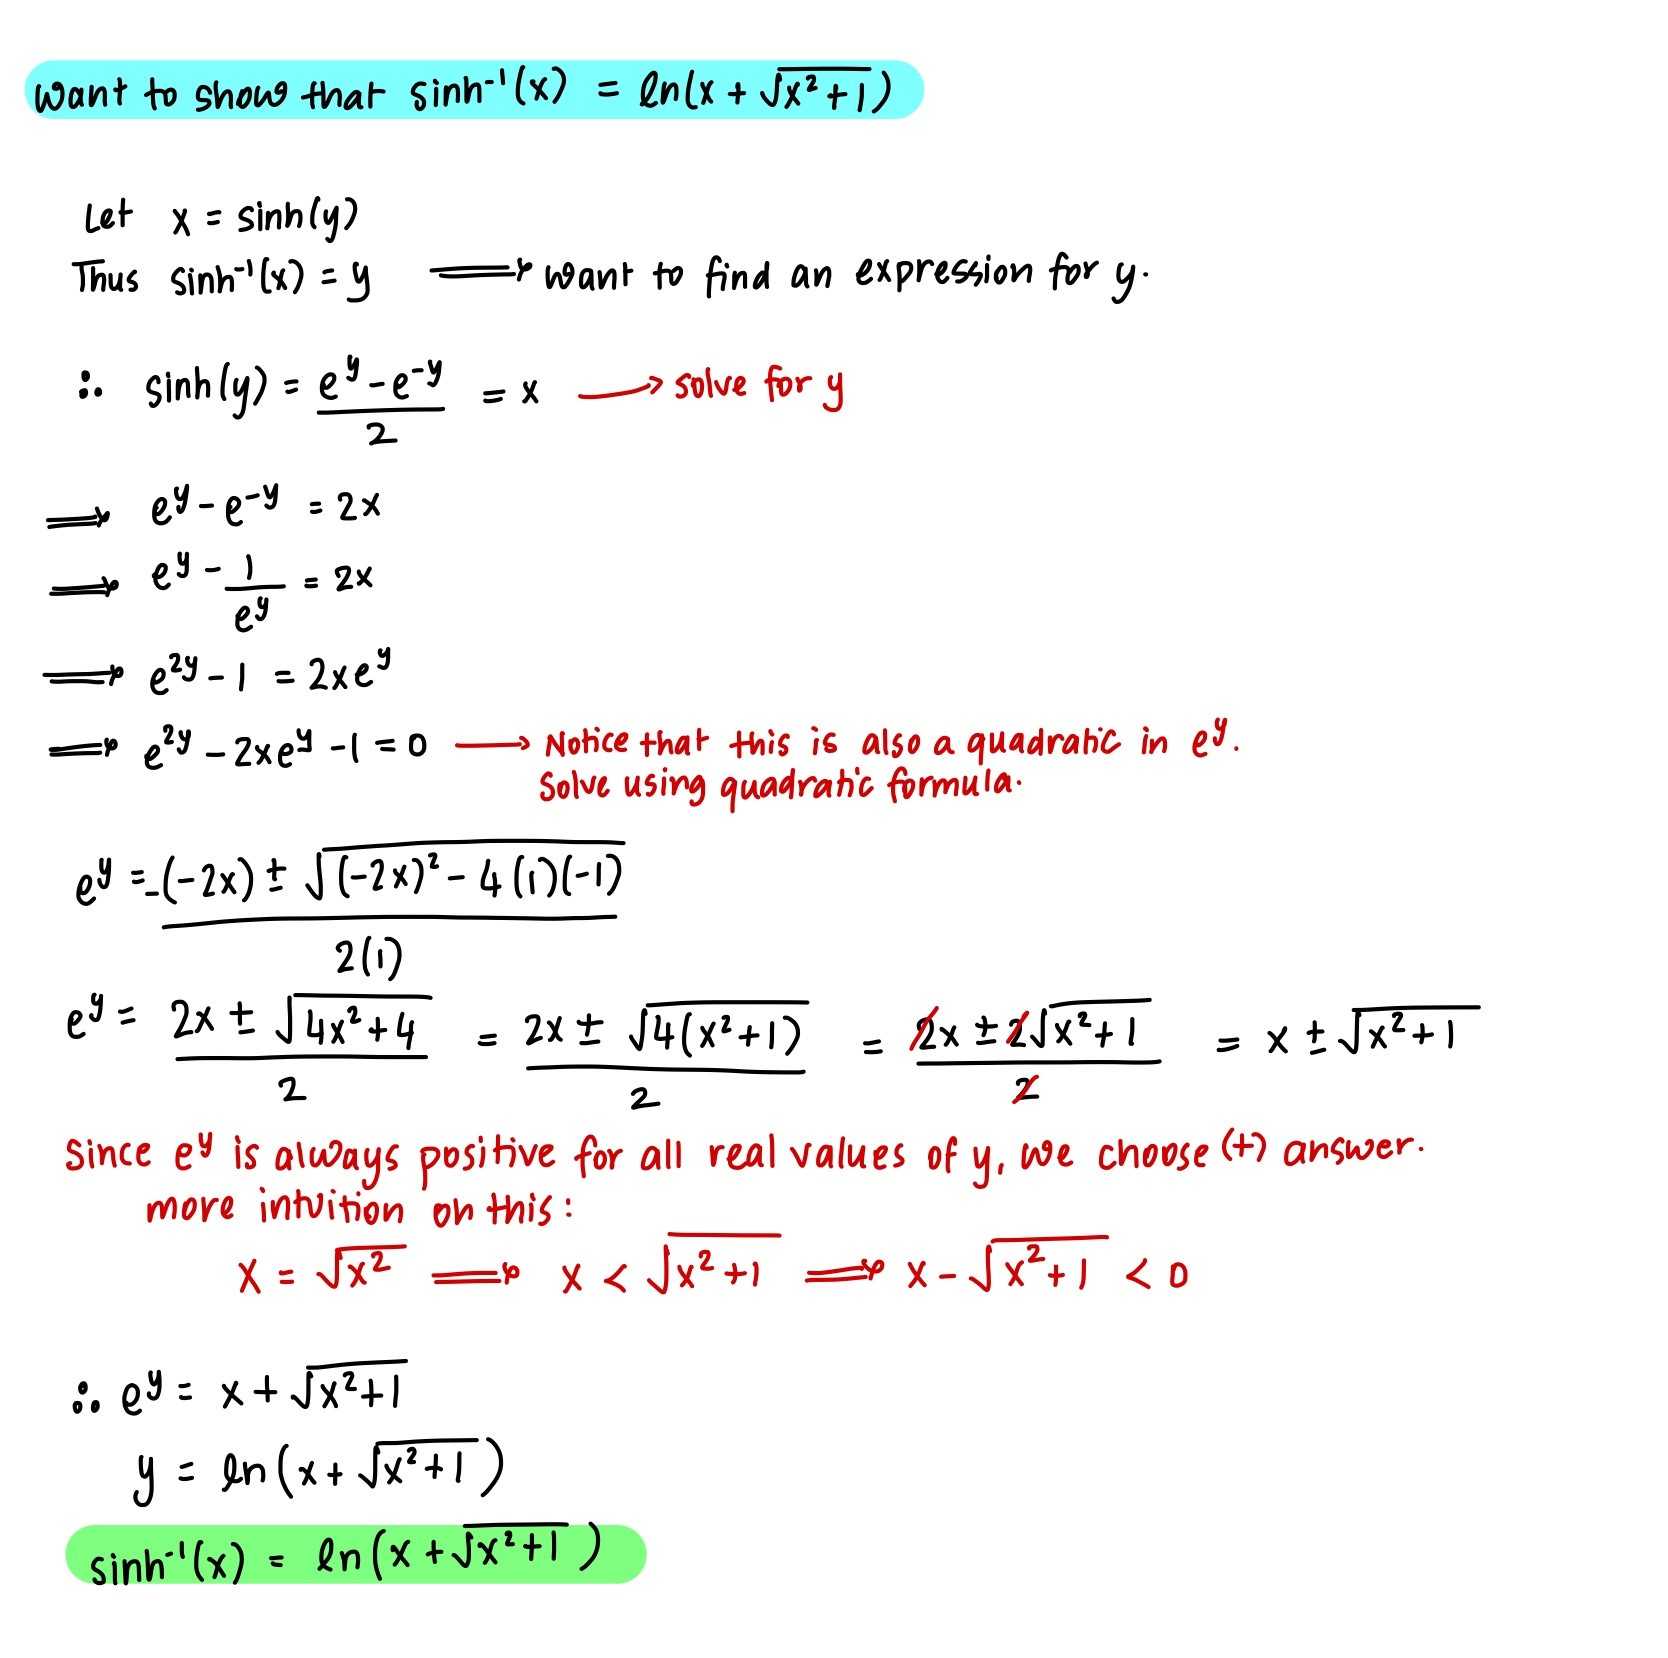
\includegraphics[width=\linewidth]{Q2.2.jpg}
        \label{fig:Q2.2}
    \end{figure}
    \newpage
    \item Find expressions for $\cosh^{-1}x$ and $\tanh^{-1}x$
    \begin{figure}[H]
        \centering
        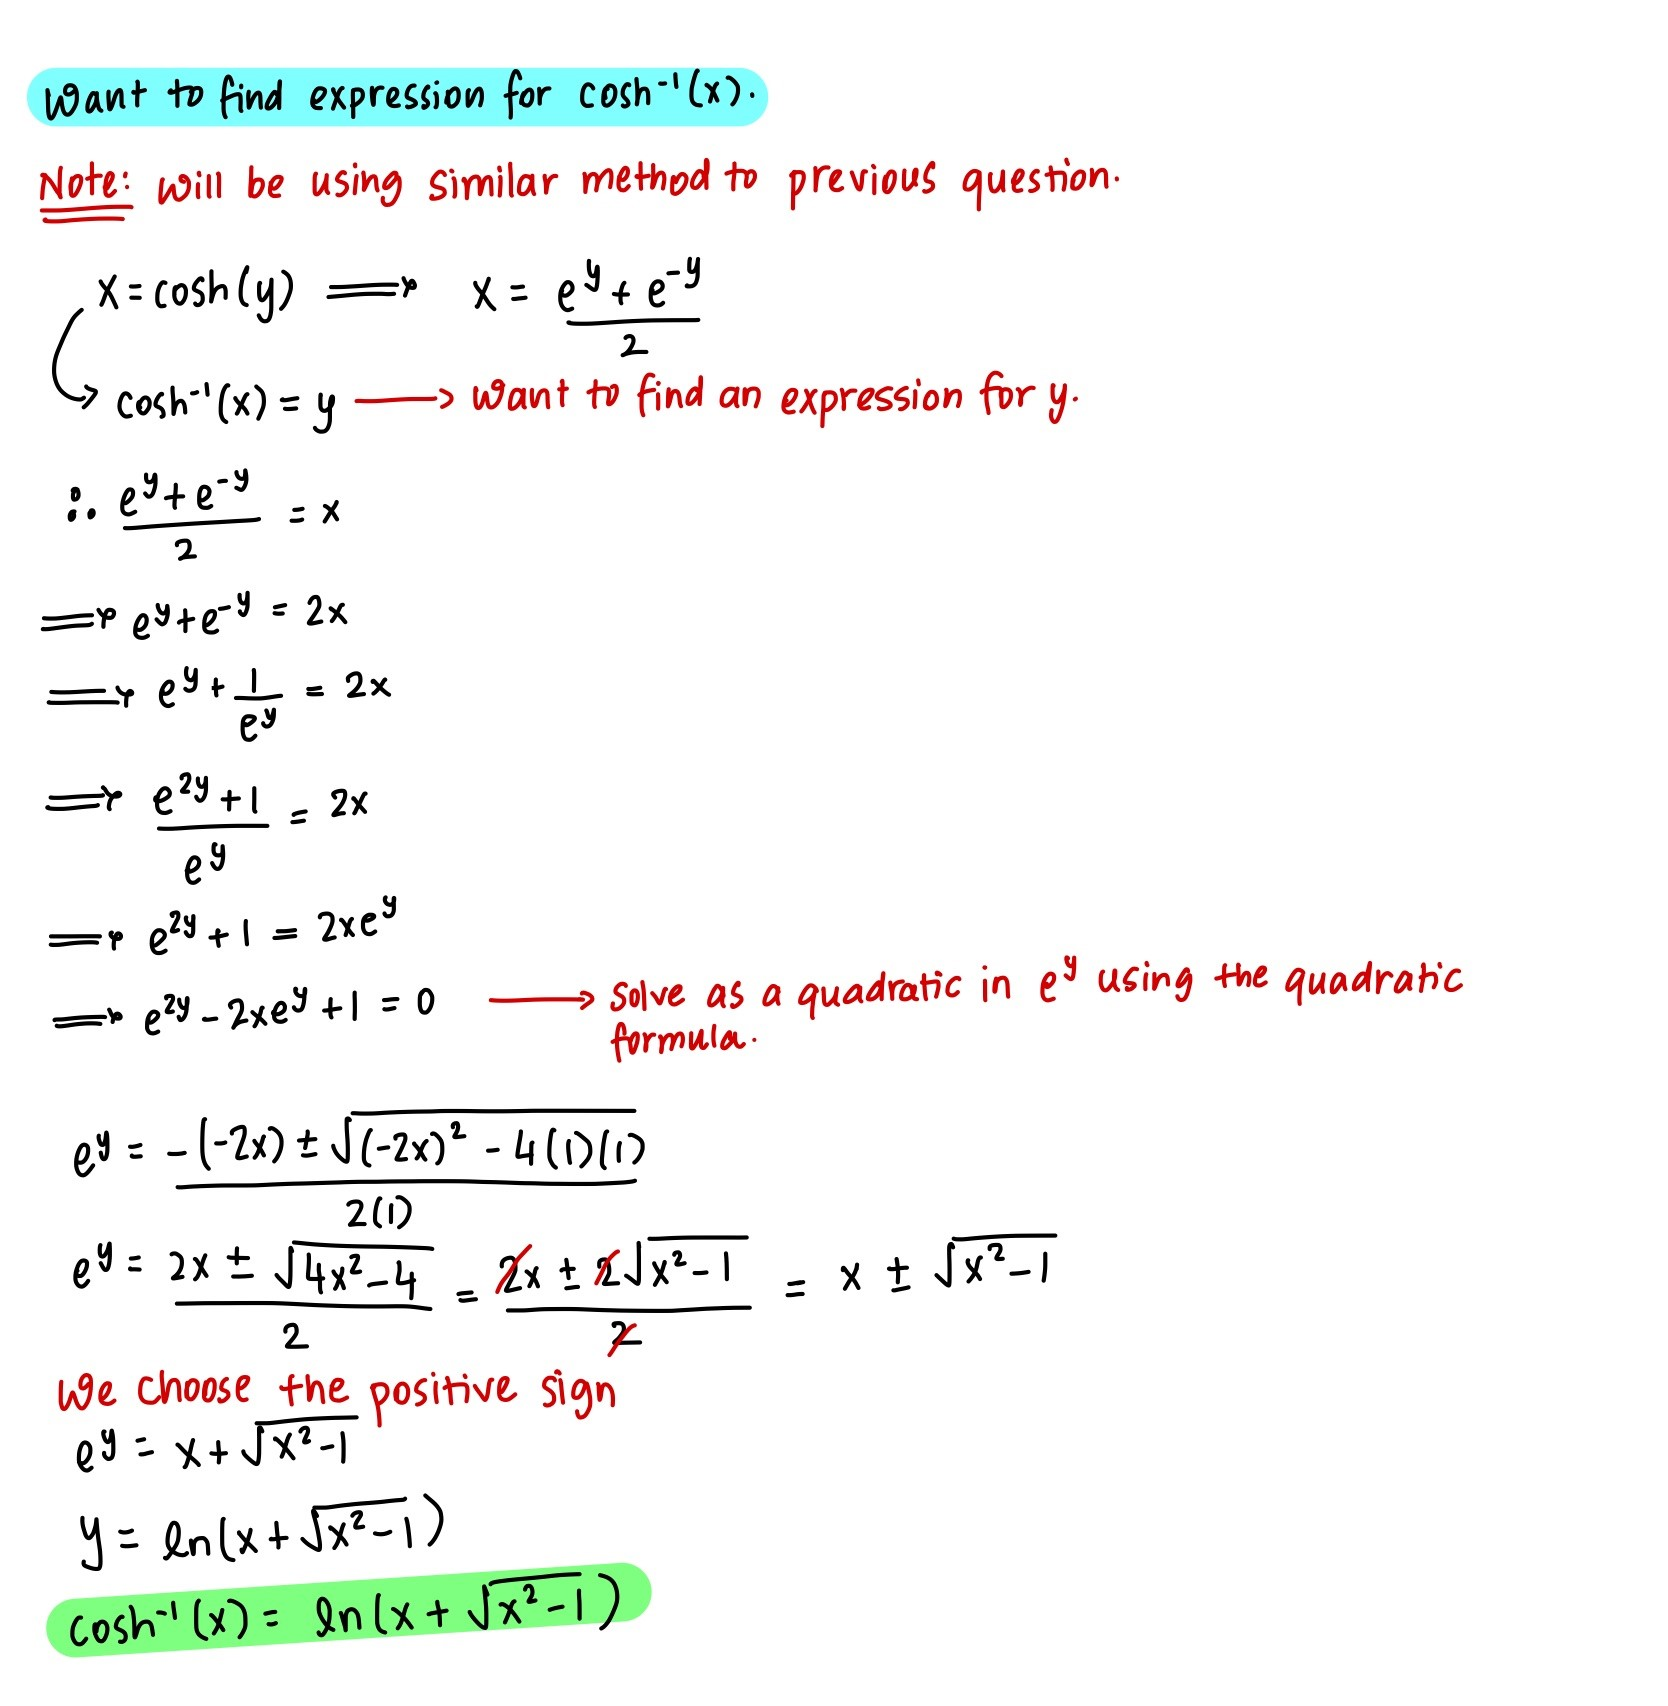
\includegraphics[width=\linewidth]{Q2.31.jpg}
        \label{fig:Q2.31}
    \end{figure}
    \begin{figure}[H]
        \centering
        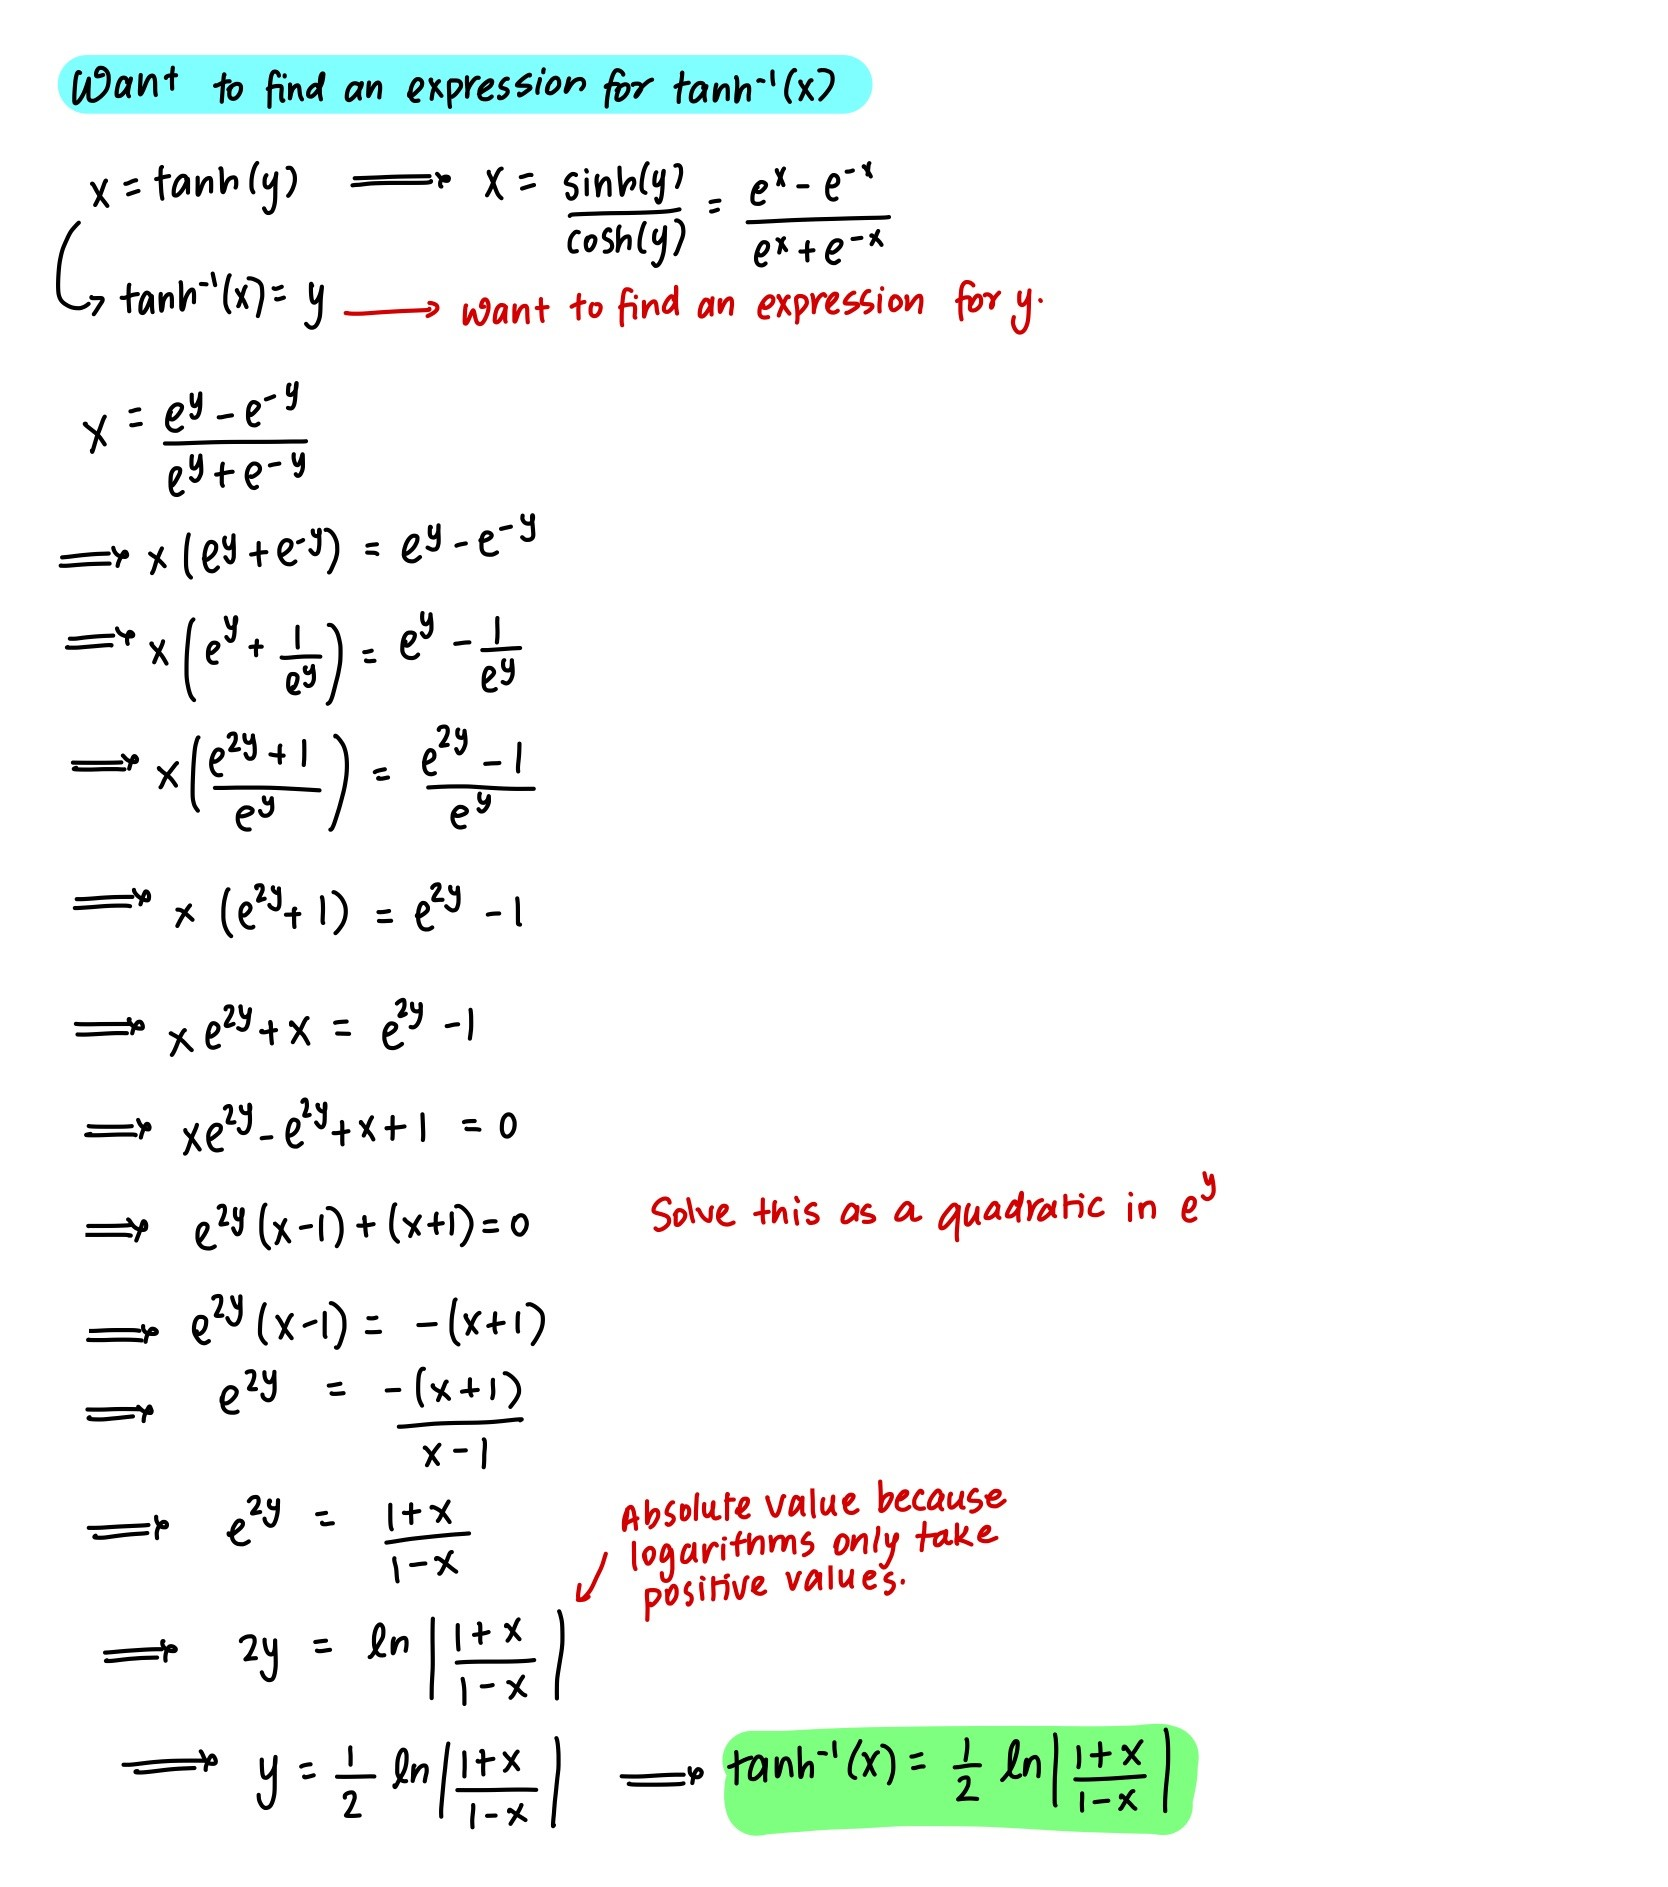
\includegraphics[width=\linewidth]{Q2.32.jpg}
        \label{fig:Q2.32}
    \end{figure}
    \newpage
    \item Find all values of $x$ that satisfy $$\sinh 2x - 3\tanh x - \sinh x = 0$$
    \begin{figure}[H]
        \centering
        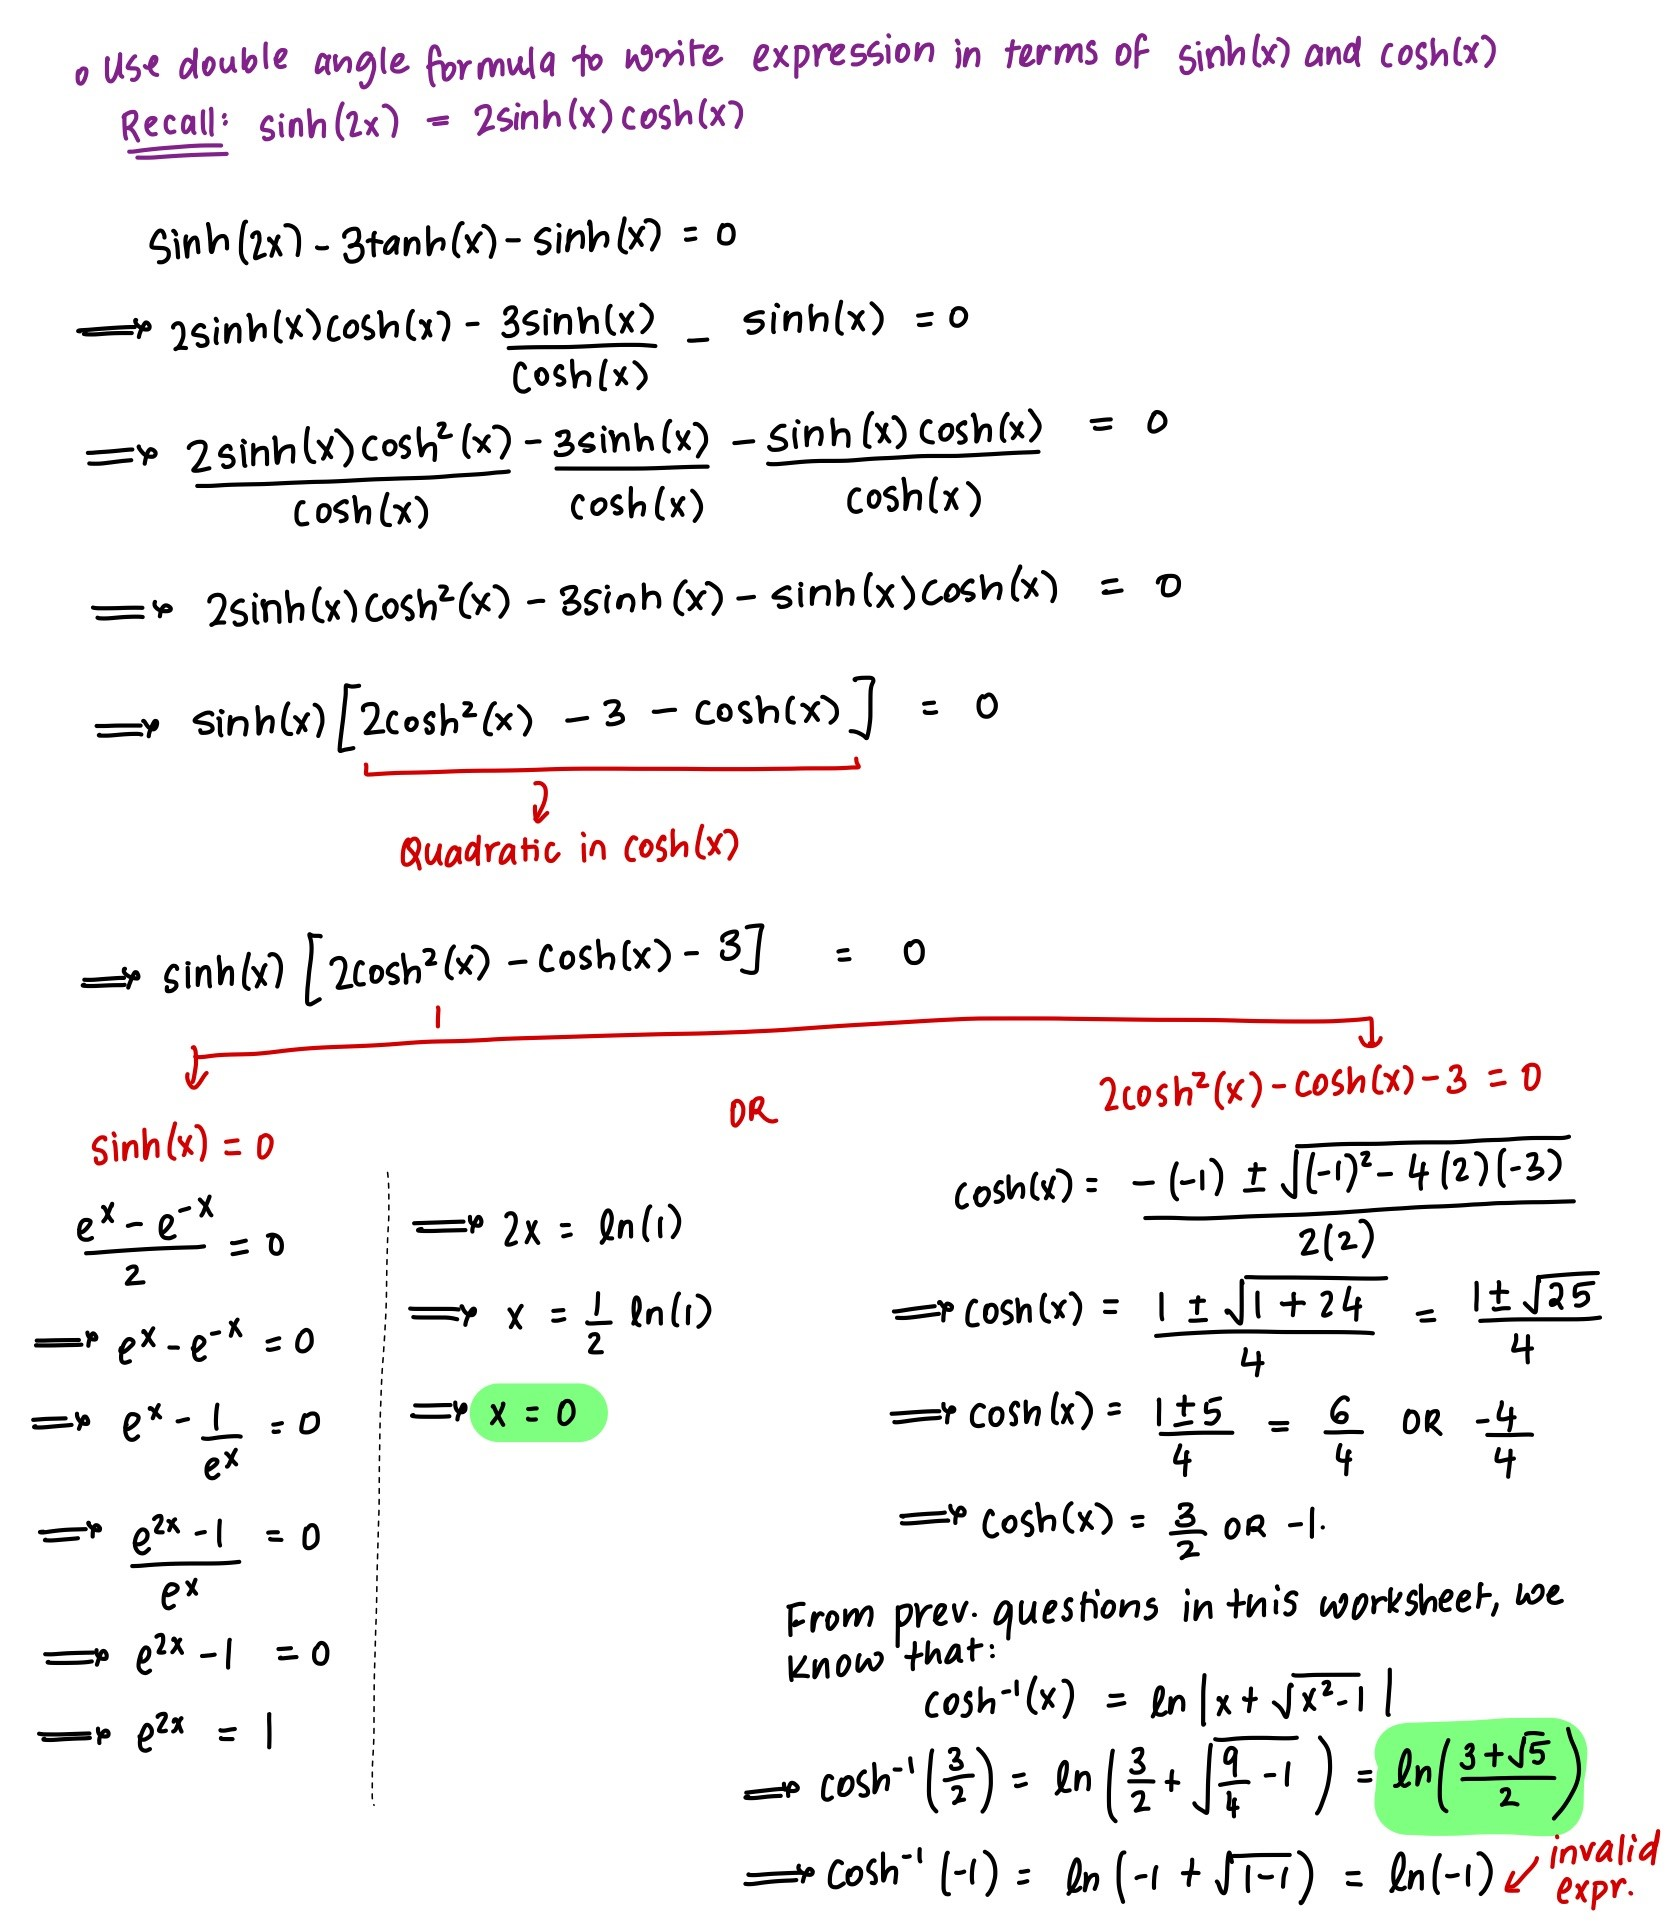
\includegraphics[width=\linewidth]{Q2.4.jpg}
        \label{fig:Q2.4}
    \end{figure}
\end{enumerate}

\end{document}

